\section{Why the ODE carries score errors and the corrected SDE forgets them}
\label{sec:forgetting}

Take a sampler with score coefficient $K$ and noise $D$ (forward-time drift $Bz-K\shat$) and a score error of the form $\shat=(1-\eta)s$ on one Gaussian mode.
The deviation $E$ of its output covariance from the true one then obeys
\begin{equation}
\begin{aligned}
&\frac{dE}{d\tau}=AE+EA^{\top}+D+G-(1-\eta)(K+K^{\top}),\\
&A=-B-(1-\eta)KC^{-1}.
\end{aligned}
\label{eq:general}
\end{equation}
For $\eta=0$ the source vanishes identically for \Sb{} ($K=\tfrac12(G+\Gp)$, $D=\Gp$) and \Sc{} ($K=\tfrac12G$, $D=0$), which recovers their exactness.
For \Sa{} ($K=D=\Gp$) it reduces to Eq.~\eqref{eq:error}.

\begin{derived}[forgetting rate]
\label{der:forgetting}
In the noise-dominated regime $C=\sigma^2I$, the relative deviation $F=E/\sigma^2$ of samplers with $K=\tfrac12(G+D)$ obeys $dF/d\tau=JF+FJ^{\top}+(\text{source})$ with
\begin{equation}
J=-\Skew B-\frac{D}{2\sigma^2}.
\label{eq:M}
\end{equation}
The source holds the injected score error; for $\eta\neq0$ it also holds the terms of order $\eta F$, so $J$ is the generator of the error-free evolution.
For the probability-flow ODE ($D=0$), $J$ is skew-symmetric: $F$ is only rotated between position and velocity, so its size $\|F\|$ (Frobenius norm) is conserved, and a relative error, once made, is never damped.
Its position component $F_{xx}$ oscillates with an amplitude that does not decay.
For the corrected SDE ($D=\Gp=2\sigma^2(r-w_{\min})\,ww^{\top}$) on the CLD block, $F$ decays at the rate $r-w_{\min}$ ($19$ at $r/\kappa=0.5$ in the setup of Sec.~\ref{sec:exact}).
\end{derived}
Equation~\eqref{eq:M} follows from $G/(2\sigma^2)=rI-\Sym B$ and $d\sigma^2/d\tau=-2r\sigma^2$.
The injected noise alone sets how fast errors are forgotten [Fig.~\ref{fig:forgetting}(a)].

\paragraph*{Comparison with the learned scores.}
We take $\eta(\sigma)=\sqrt{e(\sigma)}$ from the measured error profiles and solve Eq.~\eqref{eq:general} for \Sb{} and \Sc{}.
The predicted ratio $\Delta_{\rm iii}/\Delta_{\rm ii}$ is $6.6$ in B and $12$ in C for the final networks; the observed ratios are $6.5$ and $1.1$.
Across checkpoints [Fig.~\ref{fig:forgetting}(b)], the prediction matches setting B and the early checkpoints of C, and overestimates the later ones of C.
The predicted absolute $\Delta$ is 4--23 times too large, because the model treats the whole score error as a coherent weakening of the attraction.
We therefore claim only the ordering, $\Delta_{\rm iii}\gg\Delta_{\rm ii}$, not the magnitude.

\begin{figure}[t]
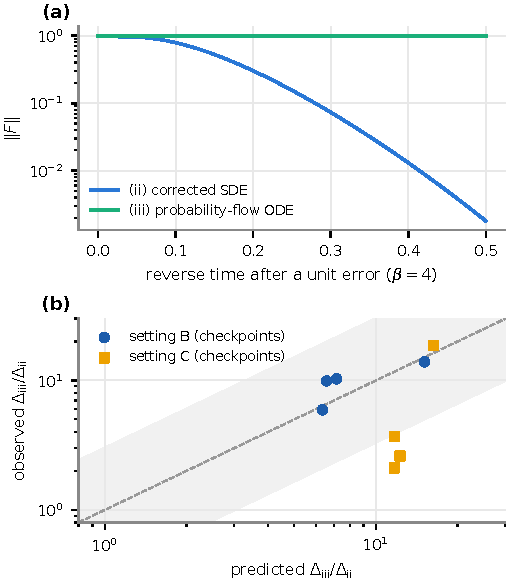
\includegraphics[width=\columnwidth]{figures/fig4_forgetting}
\caption{(a) Size of a unit relative error carried by the corrected SDE and by the probability-flow ODE in the noise-dominated regime (closed form, Eq.~\eqref{eq:M}; flow of setting B).
(b) Ratio $\Delta_{\rm iii}/\Delta_{\rm ii}$ predicted with $\shat=(1-\eta)s$, $\eta=\sqrt{e}$, against the ratio observed with learned scores over checkpoints. Shaded: within a factor of 3.}
\label{fig:forgetting}
\end{figure}
